\documentclass{beamer}
\usepackage{amsmath}
\usepackage{color}
\usepackage{ulb}
\title{Implementation of Decision Tree Classifiers\\
ID3 versus C4.5}
\author{Depuydt Antoine\\ Dany Efila \\Mudura Mircea}

\date{May, 2017}
\begin{document}
\maketitle

\addtobeamertemplate{navigation symbols}{}{%
    \usebeamerfont{footline}%
    \usebeamercolor[fg]{footline}%
    \hspace{1em}%
    \insertframenumber/\inserttotalframenumber
}

\section{Introduction}
\begin{frame}
\frametitle{Introduction}
\begin{itemize}
\item Data mining: compress, understand and predict
	\vfill
	\begin{itemize}
		\item Clustering
		\vfill
		\item Classification
		\vfill
		\item Regression
		\vfill
		\item ...
	\end{itemize}
\vfill
\item Techniques to find links
	\vfill
	\begin{itemize}
		\item Linear Regression
		\vfill
		\item Decision Trees
		\vfill
		\item Neural Networks
		\vfill
		\item ...
	\end{itemize}
\end{itemize}
\end{frame}


\begin{frame}
\frametitle{Classification}
	\begin{itemize}
		\item Classical example: play tennis today?
		\vfill
		\begin{itemize}
			\item \textbf{Features}:
			\begin{itemize}
				\item Outlook: sunny, overcast, rainy
				\vfill
				\item Temperature: hot, cool, cold
				\vfill
				\item Wind: high, weak
				\vfill
				\item Humidity: high, normal
			\end{itemize}
			\vfill
			\item \textbf{Class labels}:
				\begin{itemize}
				\item Yes
				\vfill
				\item No
				\end{itemize}			

		\end{itemize}
	\end{itemize}
\end{frame}

\begin{frame}
\frametitle{Decision Tree}
	\begin{itemize}
		\item Visual model, easily understandable
		\vfill
		\item Model: tree with \color{blue}decision \color{black}and \color{green}leaf nodes \color{black}
	\end{itemize}
	\begin{center}
		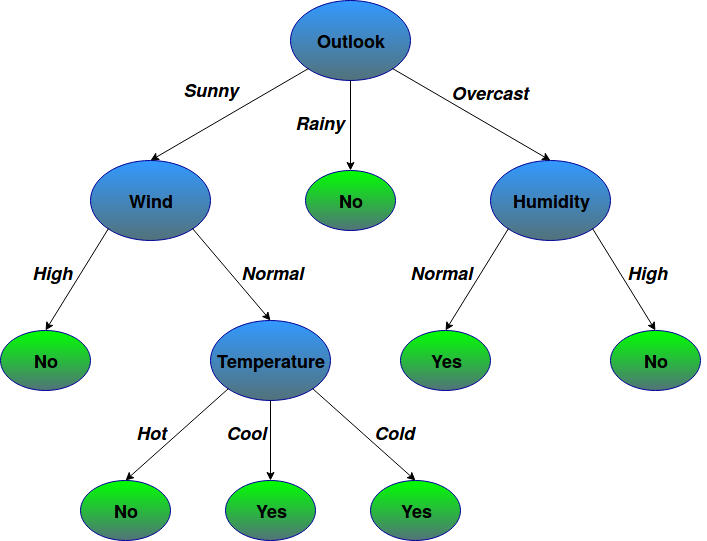
\includegraphics[scale=0.35]{Images/DecisionTree.png}
	\end{center}

\end{frame}

\begin{frame}
\frametitle{Premise}
\begin{itemize}
\item Given a training data-set 
\vfill
\item Recursively split on a node:
\vfill
\item If node is pure return leaf (class value)
\vfill
\item Else compute entropy \& info gain:
\begin{itemize}
\vfill
\item Shannon's entropy: $E(S)= \sum_{i}{} - p_i log_2(p_i) $
\vfill
\item Subtree gain: $Gain(T,X)=E(T)-E(T,X)$
\vfill
\end{itemize}
\end{itemize}
\end{frame}


\begin{frame}
\frametitle{ID3 versus C4.5}
	\begin{itemize}
		\item Goal: implement ID3 and C4.5 algorithms
		\vfill
		\item Objectives: compare ID3 and C4.5 output
		\vfill
		\begin{itemize}
			\item Compare ID3 and C4.5
			\vfill
			\item Create an application that classifies any data using both algorithms
		\end{itemize}

	\end{itemize}

\end{frame}

\begin{frame}
\frametitle{ID3}
\begin{itemize}
\item Initial implementation of decision trees
\item Top down approach
\item Split current node based on information gain:

\end{itemize}
\end{frame}

\begin{frame}
\frametitle{Improvements?}
\begin{itemize}
\item Entropy \& information gain not sufficient metrics
\vfill
\item Missing data has to be handled
\vfill
\item Numerical values could provide order or dimension to a problem set
\vfill
\item Tree can be simplified
\end{itemize}
\end{frame}

\begin{frame}[allowframebreaks]
\frametitle{Missing data}
\begin{center}
%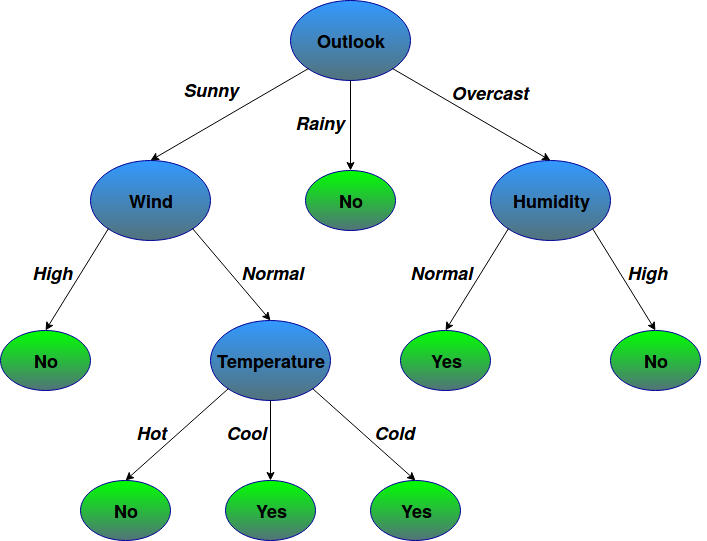
\includegraphics[scale=.1]{Images/DecisionTree.png}

2,*,*,*,*,*,2\\
1,2,*,*,*,*,1\\
1,1,2,*,*,*,1\\
1,1,1,*,*,*,1\\
1,1,3,2,2,*,1\\
1,*,*,*,*,4,1\\
2,1,4,*,*,1,1\\
2,1,4,*,*,2,1\\
2,1,4,*,*,3,1\\
2,1,3,1,1,1,1\\
2,1,3,1,1,2,1\\
2,1,3,1,2,1,1\\
2,1,3,1,2,2,1\\
1,1,3,1,1,3,1\\
2,1,3,1,2,3,1
\end{center}

\begin{itemize}
\item Dataypes can co-exist (eg. strings, integer/float)
\vfill
\item Solutions
\begin{itemize}
\item Replace missing values in column with most frequent
\item For numerical values replace with mean/mode/median
\end{itemize}
\item Column 2:
\begin{itemize}
\item No instances = 15
\item Card(2) = 1
\item Card(1) = 12
\item $\rightarrow$ safest choice replace missing values with 1 
\end{itemize}
\item Column 3:
\begin{itemize}
\item No instances = 15 (of course)
\item Card(2) = 1 
\item Card(1) = 1
\item Card(3) = 7
\item Card(4) = 3
\item Missing = 3
\item $\rightarrow$ replace missing values with 3
\end{itemize}
\end{itemize}
\end{frame}

\begin{frame}
\frametitle{Numerical \& continuous variables}
\begin{itemize}
\item General approach separate categorical and continuous
\vfill
\item Our implementation:
\begin{itemize}
\vfill
\item Treat all numerical variables as continuous
\vfill
\item C45 implementation based on  a binary tree (computational gain)
\vfill
\item $\rightarrow$ Everything equal or smaller than node value to the left
\vfill
\item $\rightarrow$ Everything else to the right
\end{itemize}
\end{itemize}
\end{frame}




\begin{frame}[allowframebreaks]
\frametitle{C4.5}
\begin{itemize}
\item Simplifying a tree
\vfill
\begin{itemize}
\item Given a target gain level (generic or user-defined)
\vfill
\item Prune (condense) the subtree
\vfill
\begin{itemize}
\item Might induce overclassification or errors
\vfill
\item Decreases the depth of the tree 
\vfill
\end{itemize}
\end{itemize}
\item 2 strategies:
\vfill
\begin{itemize}
\item \textbf{Pre-prune:}
\vfill
\begin{itemize}
\item Using statistical signifiance
\vfill
\item $\rightarrow$ stop growing/building when no statistical significant association between any attribute and class at a node
\vfill
\item chi-squared test ( too much statistics for us)
\vfill
\item Pre-pruning may stop growing prematurely (eg. XOR stops at root node)
\vfill
\end{itemize}
\framebreak
\item \textbf{Post-prune:}
\begin{itemize}
\item Subtree replacement
\vfill
\item $\rightarrow$ Replace subtree with leaf
\vfill
\item $\rightarrow$ Stop when additional pruning is harmful
\vfill
\item $\rightarrow$ Accuracy default/user given
\vfill
\item $\rightarrow$ Usinga validation test-set (derived from original)
\vfill
\item Subtree raising
\vfill
\item $\rightarrow$ Delete node \& redistribute instances
\vfill
\item $\rightarrow$ Slower than replacement strategy
\end{itemize}
\end{itemize}
\end{itemize}


\end{frame}


\begin{frame}
\frametitle{Pruning}
\begin{itemize}
\item Example avec notre code
\end{itemize}
\end{frame}

\begin{frame}
\frametitle{C4.5 - last slide, we promise}
\begin{itemize}
\item Implementation differences to ID3
\begin{itemize}
\vfill
\item First test for missing values and replace
\vfill
\item When splitting apply rule for numerical values
\vfill
\item After growing the tree: prune
\vfill
\end{itemize}
\end{itemize}
\end{frame}


\begin{frame}
\frametitle{Demonstration}
	\begin{center}
		
\includegraphics[scale=0.35]{Images/demo2.png}
	\end{center}
\end{frame}
\end{document}
